%
% $RCSfile: classification.tex,v $
%
% Copyright (c) 2004. Christian Heller. All rights reserved.
%
% No copying, altering, distribution or any other actions concerning this
% document, except after explicit permission by the author!
% At some later point in time, this document is planned to be put under
% the GNU FDL license. For now, _everything_ is _restricted_ by the author.
%
% http://www.cybop.net
% - Cybernetics Oriented Programming -
%
% http://www.resmedicinae.org
% - Information in Medicine -
%
% @author Christian Heller <christian.heller@tuxtax.de>
%

\subsection{Classification}
\label{classification_heading}

Several schemes of \emph{Pattern Classification} exist. One possible is shown in
figure \ref{pattern_figure}. Considering the level of abstraction (granularity),
it distinguishes between \emph{Architectural-}, \emph{Design-} and \emph{Idiomatic}
patterns \cite{buschmann}. Design patterns, in turn, are divided after their
functionality (problem category) into \emph{Creational-}, \emph{Structural-}
and \emph{Behavioural} patterns \cite{gamma1995}. The Wikipedia Encyclopedia
\cite{wikipedia} mentions three further problem categories: \emph{Fundamental-},
\emph{Concurrency-} and \emph{Real-time} patterns. Other criteria (dimensions)
of classification exist. Fowler introduces a completely different category which
he calls \emph{Analysis Patterns} \cite{fowler1997}. These are applicable early
in the \emph{Software Engineering Process} (SEP). And he defines patterns that
are more often used for describing the modelling \emph{Language} than the actual
\emph{Models} as \emph{Meta Model Patterns}.

\begin{figure}[ht]
    \begin{center}
        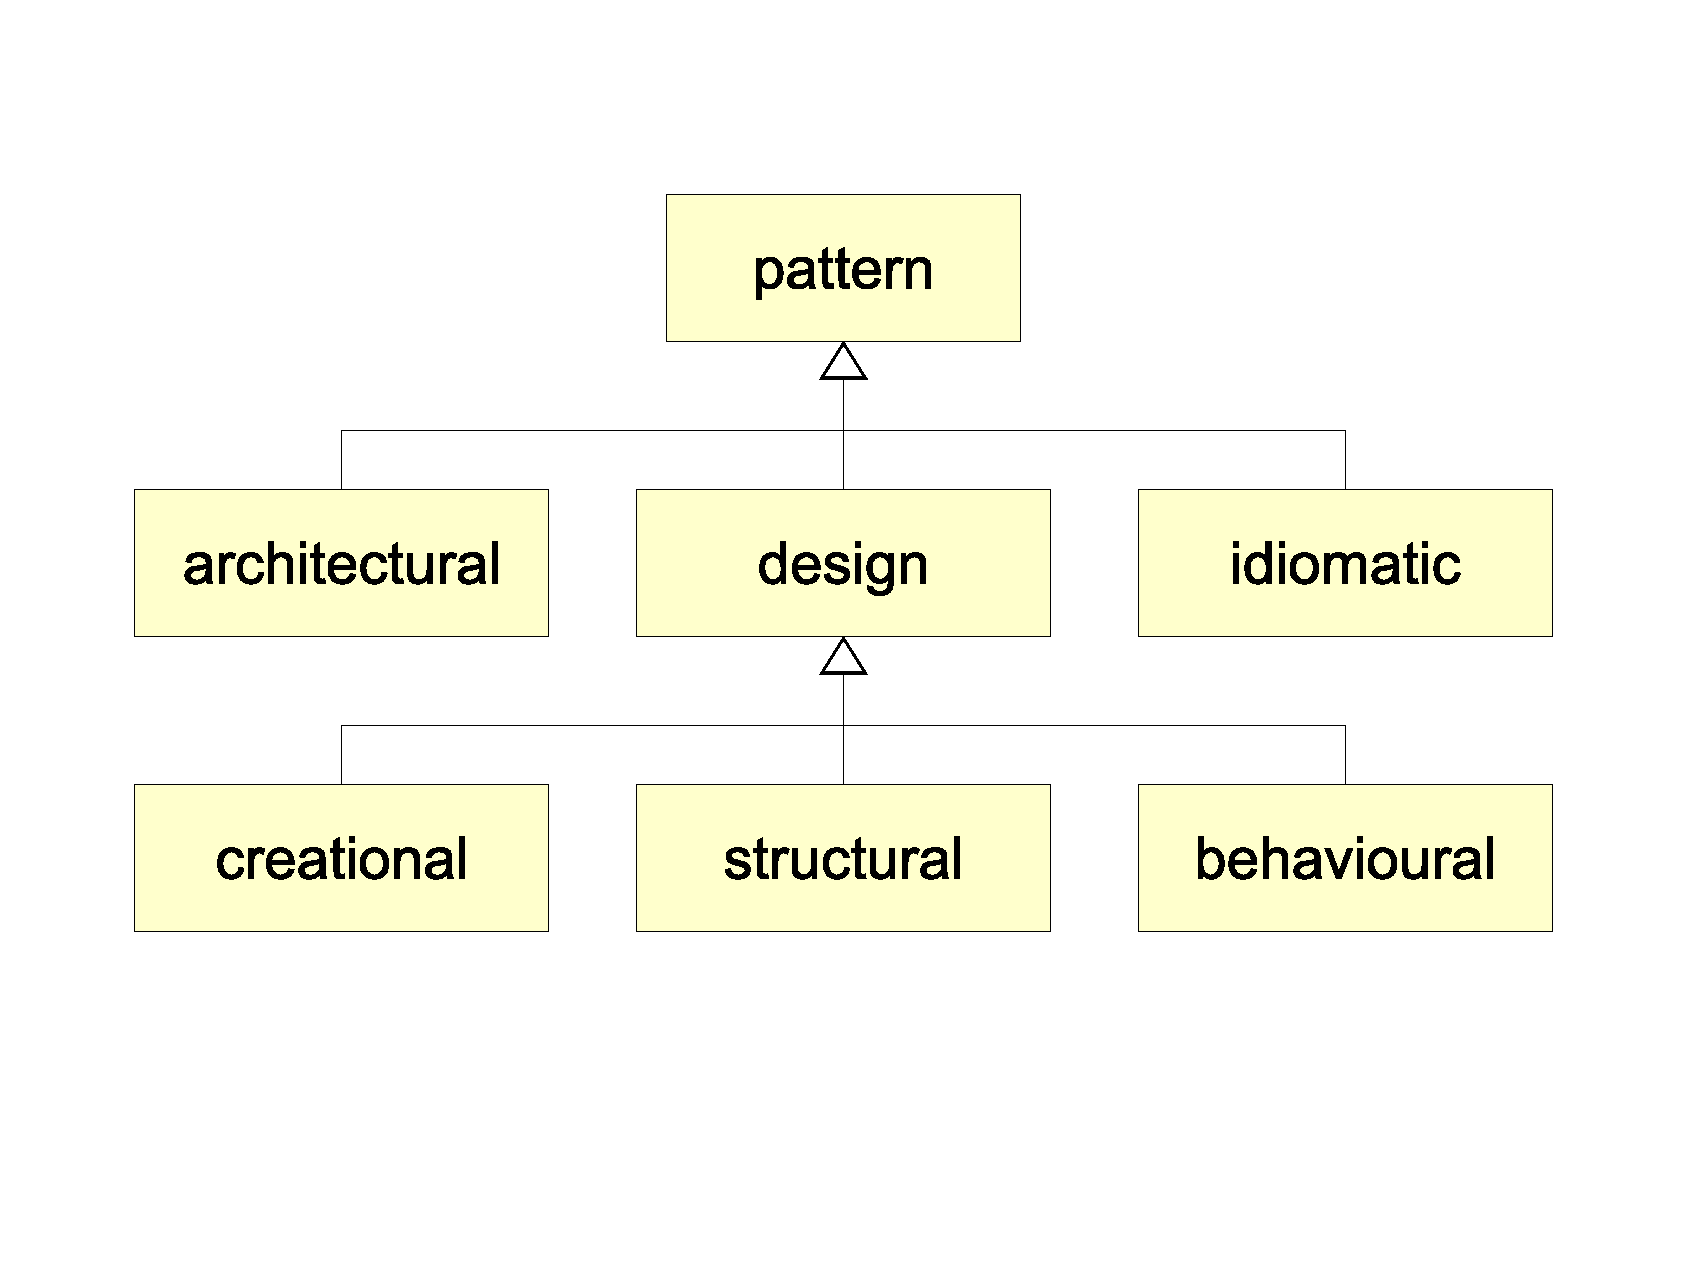
\includegraphics[scale=0.3]{vector/pattern.eps}
        \caption{Software Pattern Classification}
        \label{pattern_figure}
    \end{center}
\end{figure}
